\newcommand{\rev}{03 - 26-Mar-2021}
% REV03 Fri 26 Mar 2021 16:45:54 WIB
% REV02 Fri 26 Mar 2021 14:02:28 WIB
% REV01 Fri 26 Mar 2021 13:49:14 WIB
% START Fri 26 Mar 2021 12:10:02 WIB

\documentclass[12pt]{book}
\usepackage[a4paper, margin=50pt]{geometry}
\usepackage{colortbl}
\usepackage[pdftex]{graphicx}

\newcommand{\pengarangs}{%
    Dickens McCartney\\
}
\newcommand{\judul}{%
Jenny Wren\\[13pt]
Our Mutual Friend
}

\begin{document}

\begin{titlepage}
    \begin{center}    

    \vspace*{15mm}
    \textbf{\Large \judul}

    \vspace*{30mm}       
    \textbf{by}

    \vspace*{15mm}    
    \textbf{\Large \pengarangs}

    \vspace*{4.0cm}

    \begin{center}
        
\includegraphics[width=40mm]{ucls-coat}
    \end{center}

    \textbf{
       Universe Centra Le Sahara (UCLS)\\[11pt]
       Omar Bakry School of Management\\[11pt]
       Jabal Acacus Campus, Ghat. \\[11pt]
       Rev. \rev%
    }

    \vspace*{5mm}    
    \textbf{\LARGE \textcolor{red}{***** DRAFT *****}}

    \end{center}

\end{titlepage}

\pagenumbering{roman}

\tableofcontents

\newpage

\chapter*{Jenny Wren}
\addcontentsline{toc}{chapter}{Jenny Wren}

\begin{verbatim}
Like so many girls
Jenny Wren could sing
But a broken heart
Took her soul away

Like the other girls
Jenny Wren took wing
She could see the world
And it's foolish ways

How, we, spend our days
Casting, love aside
Loosing, site of life
Day, by, day

She saw poverty
Breaking all the home
Wounded warriors
Took her song away

But the day will come
Jenny Wren will sing
When this broken world
Mends its foolish ways

Now we, spend our days
Catching, up on life
All because of you
Jenny Wren

--- Dickens McCartney
\end{verbatim}

\noindent
Jenny Wren --- whose real name is Fanny Cleaver,
is ''the dolls' dressmaker'' with whom Lizzie lives after her father dies.
She is crippled with a bad back, although not ugly.
She is very motherly towards her drunken father, whom she calls her ''bad child''.
Jenny later cares for Eugene while he recovers from Headstone's attack on his life.
She may have a romance with Sloppy at the end of the book,
which the reader may surmise will end in marriage.
Although her mannerisms give her a certain ''strangeness'', Jenny is very perceptive,
identifying Eugene Wrayburn's intentions towards Lizzie in his small actions.
Her role is a creator and a caretaker, 
and her ''pleasant fancies'' of ''flowers, bird song, numbers of blessed, 
white-clad children'' reflect the mind's ability to rise above adverse 
circumstances --- \textbf{WikiPedia}.

\noindent
=== Rev. \rev ===

\newpage

\pagenumbering{arabic}

\part{Book the First:\\THE CUP AND THE LIP}

% REV00 Fri 26 Mar 2021 17:22:59 WIB
% START Fri 26 Mar 2021 17:22:59 WIB

\chapter{ON THE LOOK OUT}

In these times of ours, though concerning the exact year there is no
need to be precise, a boat of dirty and disreputable appearance,
with two figures in it, floated on the Thames, between Southwark
bridge which is of iron, and London Bridge which is of stone, as an
autumn evening was closing in.

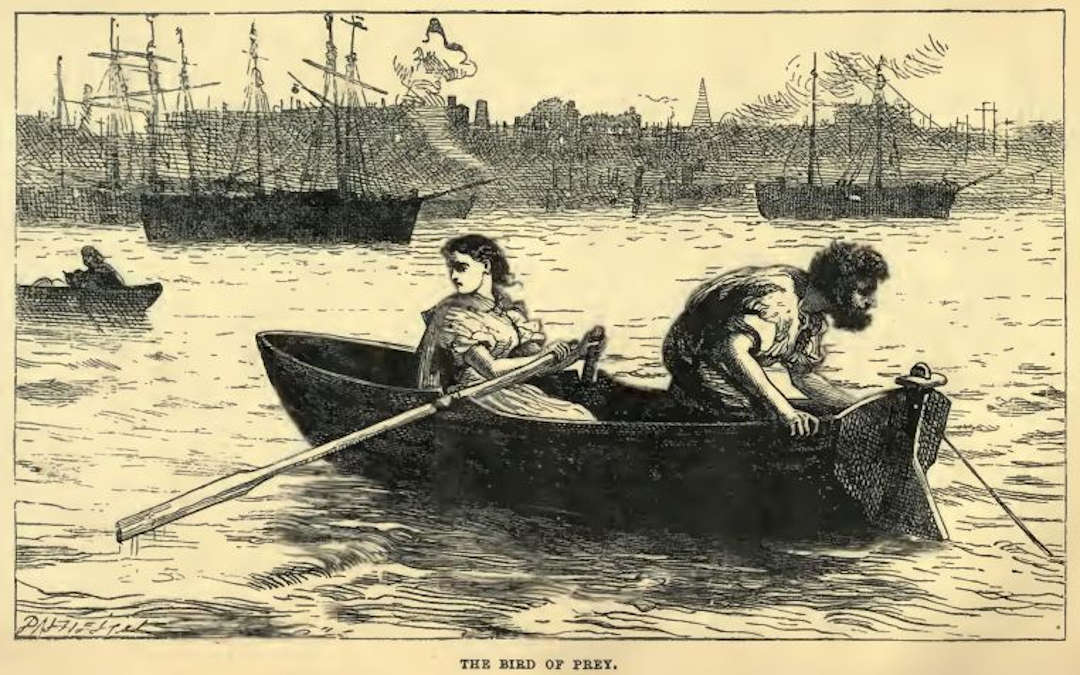
\includegraphics[scale=2.3]{01-01-01}

The figures in this boat were those of a strong man with ragged
grizzled hair and a sun-browned face, and a dark girl of nineteen or
twenty, sufficiently like him to be recognizable as his daughter.
The girl rowed, pulling a pair of sculls very easily; the man, with
the rudder-lines slack in his hands, and his hands loose in his
waistband, kept an eager look out. He had no net, hook, or line,
and he could not be a fisherman; his boat had no cushion for a
sitter, no paint, no inscription, no appliance beyond a rusty
boathook and a coil of rope, and he could not be a waterman; his
boat was too crazy and too small to take in cargo for delivery, and
he could not be a lighterman or river-carrier; there was no clue to
what he looked for, but he looked for something, with a most intent
and searching gaze. The tide, which had turned an hour before,
was running down, and his eyes watched every little race and eddy
in its broad sweep, as the boat made slight head-way against it, or
drove stern foremost before it, according as he directed his
daughter by a movement of his head. She watched his face as
earnestly as he watched the river. But, in the intensity of her look
there was a touch of dread or horror.

Allied to the bottom of the river rather than the surface, by reason
of the slime and ooze with which it was covered, and its sodden
state, this boat and the two figures in it obviously were doing
something that they often did, and were seeking what they often
sought. Half savage as the man showed, with no covering on his
matted head, with his brown arms bare to between the elbow and
the shoulder, with the loose knot of a looser kerchief lying low on
his bare breast in a wilderness of beard and whisker, with such
dress as he wore seeming to be made out of the mud that begrimed
his boat, still there was a business-like usage in his steady gaze.
So with every litle action of the girl, with every turn of her wrist,
perhaps most of all with her look of dread or horror; they were
things of usage.

'Keep her out, Lizzie. Tide runs strong here. Keep her well afore
the sweep of it.'

Trusting to the girl's skill and making no use of the rudder, he eyed
the coming tide with an absorbed attention. So the girl eyed him.
But, it happened now, that a slant of light from the setting sun
glanced into the bottom of the boat, and, touching a rotten stain
there which bore some resemblance to the outline of a muffled
human form, coloured it as though with diluted blood. This caught
the girl's eye, and she shivered.

'What ails you?' said the man, immediately aware of it, though so
intent on the advancing waters; 'I see nothing afloat.'

The red light was gone, the shudder was gone, and his gaze, which
had come back to the boat for a moment, travelled away again.
Wheresoever the strong tide met with an impediment, his gaze
paused for an instant. At every mooring-chain and rope, at every
stationery boat or barge that split the current into a broad-arrowhead,
at the offsets from the piers of Southwark Bridge, at the
paddles of the river steamboats as they beat the filthy water, at the
floating logs of timber lashed together lying off certain wharves,
his shining eyes darted a hungry look. After a darkening hour or
so, suddenly the rudder-lines tightened in his hold, and he steered
hard towards the Surrey shore.

Always watching his face, the girl instantly answered to the action
in her sculling; presently the boat swung round, quivered as from a
sudden jerk, and the upper half of the man was stretched out over
the stern.

The girl pulled the hood of a cloak she wore, over her head and
over her face, and, looking backward so that the front folds of this
hood were turned down the river, kept the boat in that direction
going before the tide.
Until now, the boat had barely held her own,
and had hovered about one spot; but now, the banks changed
swiftly, and the deepening shadows and the kindling lights of
London Bridge were passed, and the tiers of shipping lay on either
hand.

It was not until now that the upper half of the man came back into
the boat. His arms were wet and dirty, and he washed them over
the side. In his right hand he held something, and he washed that
in the river too.
It was money.
He chinked it once, and he blew
upon it once, and he spat upon it once,--'for luck,' he hoarsely said
--before he put it in his pocket.

'Lizzie!'

The girl turned her face towards him with a start, and rowed in silence.
Her face was very pale.
He was a hook-nosed man, and
with that and his bright eyes and his ruffled head, bore a certain
likeness to a roused bird of prey.

'Take that thing off your face.'

She put it back.

'Here! and give me hold of the sculls. I'll take the rest of the spell.'

'No, no, father! Father!--I cannot sit so near it!' No!
I can't indeed.

He was moving towards her to change places, but her terrified
expostulation stopped him and he resumed his seat.

‘What hurt can it do you?’

‘None, none. But I cannot bear it.’

‘It’s my belief you hate the sight of the very river.’

‘I--I do not like it, father.’

‘As if it wasn’t your living! As if it wasn’t meat and drink to you!’

At these latter words the girl shivered again, and for a moment paused
in her rowing, seeming to turn deadly faint. It escaped his attention,
for he was glancing over the stern at something the boat had in tow.

‘How can you be so thankless to your best friend, Lizzie? The very
fire that warmed you when you were a babby, was picked out of the river
alongside the coal barges. The very basket that you slept in, the tide
washed ashore. The very rockers that I put it upon to make a cradle
of it, I cut out of a piece of wood that drifted from some ship or
another.’

Lizzie took her right hand from the scull it held, and touched her
lips with it, and for a moment held it out lovingly towards him: then,
without speaking, she resumed her rowing, as another boat of similar
appearance, though in rather better trim, came out from a dark place and
dropped softly alongside.

‘In luck again, Gaffer?’ said a man with a squinting leer, who sculled
her and who was alone, ‘I know’d you was in luck again, by your wake as
you come down.’

‘Ah!’ replied the other, drily. ‘So you’re out, are you?’

‘Yes, pardner.’

There was now a tender yellow moonlight on the river, and the new comer,
keeping half his boat’s length astern of the other boat looked hard at
its track.

‘I says to myself,’ he went on, ‘directly you hove in view, yonder’s
Gaffer, and in luck again, by George if he ain’t! Scull it is,
pardner--don’t fret yourself--I didn’t touch him.’ This was in answer
to a quick impatient movement on the part of Gaffer: the speaker at the
same time unshipping his scull on that side, and laying his hand on the
gunwale of Gaffer’s boat and holding to it.

‘He’s had touches enough not to want no more, as well as I make him
out, Gaffer! Been a knocking about with a pretty many tides, ain’t he
pardner? Such is my out-of-luck ways, you see! He must have passed me
when he went up last time, for I was on the lookout below bridge here. I
a’most think you’re like the wulturs, pardner, and scent ‘em out.’

He spoke in a dropped voice, and with more than one glance at Lizzie who
had pulled on her hood again. Both men then looked with a weird unholy
interest in the wake of Gaffer’s boat.

‘Easy does it, betwixt us. Shall I take him aboard, pardner?’

‘No,’ said the other. In so surly a tone that the man, after a blank
stare, acknowledged it with the retort:

‘--Arn’t been eating nothing as has disagreed with you, have you,
pardner?’

‘Why, yes, I have,’ said Gaffer. ‘I have been swallowing too much of
that word, Pardner. I am no pardner of yours.’

‘Since when was you no pardner of mine, Gaffer Hexam Esquire?’

‘Since you was accused of robbing a man. Accused of robbing a live man!’
said Gaffer, with great indignation.

‘And what if I had been accused of robbing a dead man, Gaffer?’

‘You COULDN’T do it.’

‘Couldn’t you, Gaffer?’

‘No. Has a dead man any use for money? Is it possible for a dead man to
have money? What world does a dead man belong to? ‘Tother world. What
world does money belong to? This world. How can money be a corpse’s? Can
a corpse own it, want it, spend it, claim it, miss it? Don’t try to go
confounding the rights and wrongs of things in that way. But it’s worthy
of the sneaking spirit that robs a live man.’

‘I’ll tell you what it is--.’

‘No you won’t. I’ll tell you what it is. You got off with a short time
of it for putting your hand in the pocket of a sailor, a live sailor.
Make the most of it and think yourself lucky, but don’t think after
that to come over ME with your pardners. We have worked together in time
past, but we work together no more in time present nor yet future. Let
go. Cast off!’

‘Gaffer! If you think to get rid of me this way--.’

‘If I don’t get rid of you this way, I’ll try another, and chop you over
the fingers with the stretcher, or take a pick at your head with the
boat-hook. Cast off! Pull you, Lizzie. Pull home, since you won’t let
your father pull.’

Lizzie shot ahead, and the other boat fell astern. Lizzie’s father,
composing himself into the easy attitude of one who had asserted the
high moralities and taken an unassailable position, slowly lighted a
pipe, and smoked, and took a survey of what he had in tow. What he had
in tow, lunged itself at him sometimes in an awful manner when the boat
was checked, and sometimes seemed to try to wrench itself away, though
for the most part it followed submissively. A neophyte might have
fancied that the ripples passing over it were dreadfully like faint
changes of expression on a sightless face; but Gaffer was no neophyte
and had no fancies.


% REV00 Fri 26 Mar 2021 18:30:59 WIB
% START Fri 26 Mar 2021 18:30:49 WIB

\chapter{THE MAN FROM SOMEWHERE}

Mr and Mrs Veneering were bran-new people in a bran-new house in a
bran-new quarter of London. Everything about the Veneerings was spick
and span new. All their furniture was new, all their friends were new,
all their servants were new, their plate was new, their carriage was
new, their harness was new, their horses were new, their pictures
were new, they themselves were new, they were as newly married as was
lawfully compatible with their having a bran-new baby, and if they had
set up a great-grandfather, he would have come home in matting from the
Pantechnicon, without a scratch upon him, French polished to the crown
of his head.

For, in the Veneering establishment, from the hall-chairs with the new
coat of arms, to the grand pianoforte with the new action, and upstairs
again to the new fire-escape, all things were in a state of high varnish
and polish. And what was observable in the furniture, was observable in
the Veneerings--the surface smelt a little too much of the workshop and
was a trifle sticky.

There was an innocent piece of dinner-furniture that went upon easy
castors and was kept over a livery stable-yard in Duke Street, Saint
James’s, when not in use, to whom the Veneerings were a source of blind
confusion. The name of this article was Twemlow. Being first cousin
to Lord Snigsworth, he was in frequent requisition, and at many houses
might be said to represent the dining-table in its normal state. Mr and
Mrs Veneering, for example, arranging a dinner, habitually started with
Twemlow, and then put leaves in him, or added guests to him. Sometimes,
the table consisted of Twemlow and half a dozen leaves; sometimes, of
Twemlow and a dozen leaves; sometimes, Twemlow was pulled out to his
utmost extent of twenty leaves. Mr and Mrs Veneering on occasions of
ceremony faced each other in the centre of the board, and thus the
parallel still held; for, it always happened that the more Twemlow was
pulled out, the further he found himself from the center, and nearer
to the sideboard at one end of the room, or the window-curtains at the
other.

But, it was not this which steeped the feeble soul of Twemlow in
confusion. This he was used to, and could take soundings of. The abyss
to which he could find no bottom, and from which started forth the
engrossing and ever-swelling difficulty of his life, was the insoluble
question whether he was Veneering’s oldest friend, or newest friend.
To the excogitation of this problem, the harmless gentleman had devoted
many anxious hours, both in his lodgings over the livery stable-yard,
and in the cold gloom, favourable to meditation, of Saint James’s
Square. Thus. Twemlow had first known Veneering at his club, where
Veneering then knew nobody but the man who made them known to one
another, who seemed to be the most intimate friend he had in the world,
and whom he had known two days--the bond of union between their souls,
the nefarious conduct of the committee respecting the cookery of
a fillet of veal, having been accidentally cemented at that date.
Immediately upon this, Twemlow received an invitation to dine with
Veneering, and dined: the man being of the party. Immediately upon
that, Twemlow received an invitation to dine with the man, and dined:
Veneering being of the party. At the man’s were a Member, an Engineer, a
Payer-off of the National Debt, a Poem on Shakespeare, a Grievance, and
a Public Office, who all seem to be utter strangers to Veneering. And
yet immediately after that, Twemlow received an invitation to dine at
Veneerings, expressly to meet the Member, the Engineer, the Payer-off
of the National Debt, the Poem on Shakespeare, the Grievance, and the
Public Office, and, dining, discovered that all of them were the most
intimate friends Veneering had in the world, and that the wives of all
of them (who were all there) were the objects of Mrs Veneering’s most
devoted affection and tender confidence.

Thus it had come about, that Mr Twemlow had said to himself in his
lodgings, with his hand to his forehead: ‘I must not think of this. This
is enough to soften any man’s brain,’--and yet was always thinking of
it, and could never form a conclusion.

This evening the Veneerings give a banquet. Eleven leaves in the
Twemlow; fourteen in company all told. Four pigeon-breasted retainers in
plain clothes stand in line in the hall. A fifth retainer, proceeding up
the staircase with a mournful air--as who should say, ‘Here is another
wretched creature come to dinner; such is life!’--announces, ‘Mis-ter
Twemlow!’

Mrs Veneering welcomes her sweet Mr Twemlow. Mr Veneering welcomes
his dear Twemlow. Mrs Veneering does not expect that Mr Twemlow can in
nature care much for such insipid things as babies, but so old a friend
must please to look at baby. ‘Ah! You will know the friend of your
family better, Tootleums,’ says Mr Veneering, nodding emotionally at
that new article, ‘when you begin to take notice.’ He then begs to make
his dear Twemlow known to his two friends, Mr Boots and Mr Brewer--and
clearly has no distinct idea which is which.

But now a fearful circumstance occurs.

‘Mis-ter and Mis-sus Podsnap!’

‘My dear,’ says Mr Veneering to Mrs Veneering, with an air of much
friendly interest, while the door stands open, ‘the Podsnaps.’

A too, too smiling large man, with a fatal freshness on him, appearing
with his wife, instantly deserts his wife and darts at Twemlow with:

‘How do you do? So glad to know you. Charming house you have here. I
hope we are not late. So glad of the opportunity, I am sure!’

When the first shock fell upon him, Twemlow twice skipped back in
his neat little shoes and his neat little silk stockings of a bygone
fashion, as if impelled to leap over a sofa behind him; but the large
man closed with him and proved too strong.

‘Let me,’ says the large man, trying to attract the attention of his
wife in the distance, ‘have the pleasure of presenting Mrs Podsnap
to her host. She will be,’ in his fatal freshness he seems to find
perpetual verdure and eternal youth in the phrase, ‘she will be so glad
of the opportunity, I am sure!’

In the meantime, Mrs Podsnap, unable to originate a mistake on her own
account, because Mrs Veneering is the only other lady there, does her
best in the way of handsomely supporting her husband’s, by looking
towards Mr Twemlow with a plaintive countenance and remarking to Mrs
Veneering in a feeling manner, firstly, that she fears he has been
rather bilious of late, and, secondly, that the baby is already very
like him.

It is questionable whether any man quite relishes being mistaken for
any other man; but, Mr Veneering having this very evening set up the
shirt-front of the young Antinous in new worked cambric just come home,
is not at all complimented by being supposed to be Twemlow, who is dry
and weazen and some thirty years older. Mrs Veneering equally resents
the imputation of being the wife of Twemlow. As to Twemlow, he is
so sensible of being a much better bred man than Veneering, that he
considers the large man an offensive ass.

In this complicated dilemma, Mr Veneering approaches the large man with
extended hand and, smilingly assures that incorrigible personage that he
is delighted to see him: who in his fatal freshness instantly replies:

‘Thank you. I am ashamed to say that I cannot at this moment recall
where we met, but I am so glad of this opportunity, I am sure!’

Then pouncing upon Twemlow, who holds back with all his feeble might, he
is haling him off to present him, as Veneering, to Mrs Podsnap, when the
arrival of more guests unravels the mistake. Whereupon, having re-shaken
hands with Veneering as Veneering, he re-shakes hands with Twemlow as
Twemlow, and winds it all up to his own perfect satisfaction by saying
to the last-named, ‘Ridiculous opportunity--but so glad of it, I am
sure!’

Now, Twemlow having undergone this terrific experience, having likewise
noted the fusion of Boots in Brewer and Brewer in Boots, and having
further observed that of the remaining seven guests four discrete
characters enter with wandering eyes and wholly declined to commit
themselves as to which is Veneering, until Veneering has them in his
grasp;--Twemlow having profited by these studies, finds his brain
wholesomely hardening as he approaches the conclusion that he really is
Veneering’s oldest friend, when his brain softens again and all is
lost, through his eyes encountering Veneering and the large man linked
together as twin brothers in the back drawing-room near the conservatory
door, and through his ears informing him in the tones of Mrs Veneering
that the same large man is to be baby’s godfather.

‘Dinner is on the table!’

Thus the melancholy retainer, as who should say, ‘Come down and be
poisoned, ye unhappy children of men!’

Twemlow, having no lady assigned him, goes down in the rear, with
his hand to his forehead. Boots and Brewer, thinking him indisposed,
whisper, ‘Man faint. Had no lunch.’ But he is only stunned by the
unvanquishable difficulty of his existence.

Revived by soup, Twemlow discourses mildly of the Court Circular with
Boots and Brewer. Is appealed to, at the fish stage of the banquet, by
Veneering, on the disputed question whether his cousin Lord Snigsworth
is in or out of town? Gives it that his cousin is out of town. ‘At
Snigsworthy Park?’ Veneering inquires. ‘At Snigsworthy,’ Twemlow
rejoins. Boots and Brewer regard this as a man to be cultivated; and
Veneering is clear that he is a remunerative article. Meantime the
retainer goes round, like a gloomy Analytical Chemist: always seeming
to say, after ‘Chablis, sir?’--‘You wouldn’t if you knew what it’s made
of.’

The great looking-glass above the sideboard, reflects the table and the
company. Reflects the new Veneering crest, in gold and eke in silver,
frosted and also thawed, a camel of all work. The Heralds’ College found
out a Crusading ancestor for Veneering who bore a camel on his shield
(or might have done it if he had thought of it), and a caravan of camels
take charge of the fruits and flowers and candles, and kneel down be
loaded with the salt. Reflects Veneering; forty, wavy-haired, dark,
tending to corpulence, sly, mysterious, filmy--a kind of sufficiently
well-looking veiled-prophet, not prophesying. Reflects Mrs Veneering;
fair, aquiline-nosed and fingered, not so much light hair as she might
have, gorgeous in raiment and jewels, enthusiastic, propitiatory,
conscious that a corner of her husband’s veil is over herself. Reflects
Podsnap; prosperously feeding, two little light-coloured wiry wings, one
on either side of his else bald head, looking as like his hairbrushes as
his hair, dissolving view of red beads on his forehead, large allowance
of crumpled shirt-collar up behind. Reflects Mrs Podsnap; fine woman
for Professor Owen, quantity of bone, neck and nostrils like a
rocking-horse, hard features, majestic head-dress in which Podsnap has
hung golden offerings. Reflects Twemlow; grey, dry, polite, susceptible
to east wind, First-Gentleman-in-Europe collar and cravat, cheeks drawn
in as if he had made a great effort to retire into himself some years
ago, and had got so far and had never got any farther. Reflects mature
young lady; raven locks, and complexion that lights up well when well
powdered--as it is--carrying on considerably in the captivation of
mature young gentleman; with too much nose in his face, too much ginger
in his whiskers, too much torso in his waistcoat, too much sparkle in
his studs, his eyes, his buttons, his talk, and his teeth. Reflects
charming old Lady Tippins on Veneering’s right; with an immense obtuse
drab oblong face, like a face in a tablespoon, and a dyed Long Walk up
the top of her head, as a convenient public approach to the bunch of
false hair behind, pleased to patronize Mrs Veneering opposite, who
is pleased to be patronized. Reflects a certain ‘Mortimer’, another
of Veneering’s oldest friends; who never was in the house before,
and appears not to want to come again, who sits disconsolate on Mrs
Veneering’s left, and who was inveigled by Lady Tippins (a friend of
his boyhood) to come to these people’s and talk, and who won’t talk.
Reflects Eugene, friend of Mortimer; buried alive in the back of his
chair, behind a shoulder--with a powder-epaulette on it--of the mature
young lady, and gloomily resorting to the champagne chalice whenever
proffered by the Analytical Chemist. Lastly, the looking-glass reflects
Boots and Brewer, and two other stuffed Buffers interposed between the
rest of the company and possible accidents.

The Veneering dinners are excellent dinners--or new people wouldn’t
come--and all goes well. Notably, Lady Tippins has made a series of
experiments on her digestive functions, so extremely complicated and
daring, that if they could be published with their results it might
benefit the human race. Having taken in provisions from all parts of the
world, this hardy old cruiser has last touched at the North Pole, when,
as the ice-plates are being removed, the following words fall from her:

‘I assure you, my dear Veneering--’

(Poor Twemlow’s hand approaches his forehead, for it would seem now,
that Lady Tippins is going to be the oldest friend.)

‘I assure you, my dear Veneering, that it is the oddest affair! Like
the advertising people, I don’t ask you to trust me, without offering
a respectable reference. Mortimer there, is my reference, and knows all
about it.’

Mortimer raises his drooping eyelids, and slightly opens his mouth. But
a faint smile, expressive of ‘What’s the use!’ passes over his face, and
he drops his eyelids and shuts his mouth.

‘Now, Mortimer,’ says Lady Tippins, rapping the sticks of her closed
green fan upon the knuckles of her left hand--which is particularly rich
in knuckles, ‘I insist upon your telling all that is to be told about
the man from Jamaica.’

‘Give you my honour I never heard of any man from Jamaica, except the
man who was a brother,’ replies Mortimer.

‘Tobago, then.’

‘Nor yet from Tobago.’

‘Except,’ Eugene strikes in: so unexpectedly that the mature young lady,
who has forgotten all about him, with a start takes the epaulette out
of his way: ‘except our friend who long lived on rice-pudding and
isinglass, till at length to his something or other, his physician said
something else, and a leg of mutton somehow ended in daygo.’

A reviving impression goes round the table that Eugene is coming out. An
unfulfilled impression, for he goes in again.

‘Now, my dear Mrs Veneering,’ quoth Lady Tippins, I appeal to you
whether this is not the basest conduct ever known in this world? I carry
my lovers about, two or three at a time, on condition that they are very
obedient and devoted; and here is my oldest lover-in-chief, the head of
all my slaves, throwing off his allegiance before company! And here is
another of my lovers, a rough Cymon at present certainly, but of whom
I had most hopeful expectations as to his turning out well in course of
time, pretending that he can’t remember his nursery rhymes! On purpose
to annoy me, for he knows how I doat upon them!’

A grisly little fiction concerning her lovers is Lady Tippins’s point.
She is always attended by a lover or two, and she keeps a little list
of her lovers, and she is always booking a new lover, or striking out an
old lover, or putting a lover in her black list, or promoting a lover to
her blue list, or adding up her lovers, or otherwise posting her book.
Mrs Veneering is charmed by the humour, and so is Veneering. Perhaps it
is enhanced by a certain yellow play in Lady Tippins’s throat, like the
legs of scratching poultry.

‘I banish the false wretch from this moment, and I strike him out of
my Cupidon (my name for my Ledger, my dear,) this very night. But I am
resolved to have the account of the man from Somewhere, and I beg you
to elicit it for me, my love,’ to Mrs Veneering, ‘as I have lost my own
influence. Oh, you perjured man!’ This to Mortimer, with a rattle of her
fan.

‘We are all very much interested in the man from Somewhere,’ Veneering
observes.

Then the four Buffers, taking heart of grace all four at once, say:

‘Deeply interested!’

‘Quite excited!’

‘Dramatic!’

‘Man from Nowhere, perhaps!’

And then Mrs Veneering--for the Lady Tippins’s winning wiles are
contagious--folds her hands in the manner of a supplicating child, turns
to her left neighbour, and says, ‘Tease! Pay! Man from Tumwhere!’ At
which the four Buffers, again mysteriously moved all four at once,
explain, ‘You can’t resist!’

‘Upon my life,’ says Mortimer languidly, ‘I find it immensely
embarrassing to have the eyes of Europe upon me to this extent, and my
only consolation is that you will all of you execrate Lady Tippins in
your secret hearts when you find, as you inevitably will, the man from
Somewhere a bore. Sorry to destroy romance by fixing him with a local
habitation, but he comes from the place, the name of which escapes me,
but will suggest itself to everybody else here, where they make the
wine.’

Eugene suggests ‘Day and Martin’s.’

‘No, not that place,’ returns the unmoved Mortimer, ‘that’s where they
make the Port. My man comes from the country where they make the Cape
Wine. But look here, old fellow; its not at all statistical and it’s
rather odd.’

It is always noticeable at the table of the Veneerings, that no man
troubles himself much about the Veneerings themselves, and that any
one who has anything to tell, generally tells it to anybody else in
preference.

‘The man,’ Mortimer goes on, addressing Eugene, ‘whose name is Harmon,
was only son of a tremendous old rascal who made his money by Dust.’

‘Red velveteens and a bell?’ the gloomy Eugene inquires.

‘And a ladder and basket if you like. By which means, or by others, he
grew rich as a Dust Contractor, and lived in a hollow in a hilly country
entirely composed of Dust. On his own small estate the growling old
vagabond threw up his own mountain range, like an old volcano, and its
geological formation was Dust. Coal-dust, vegetable-dust, bone-dust,
crockery dust, rough dust and sifted dust,--all manner of Dust.’

A passing remembrance of Mrs Veneering, here induces Mortimer to address
his next half-dozen words to her; after which he wanders away again,
tries Twemlow and finds he doesn’t answer, ultimately takes up with the
Buffers who receive him enthusiastically.

‘The moral being--I believe that’s the right expression--of this
exemplary person, derived its highest gratification from anathematizing
his nearest relations and turning them out of doors. Having begun (as
was natural) by rendering these attentions to the wife of his bosom,
he next found himself at leisure to bestow a similar recognition on the
claims of his daughter. He chose a husband for her, entirely to his own
satisfaction and not in the least to hers, and proceeded to settle upon
her, as her marriage portion, I don’t know how much Dust, but something
immense. At this stage of the affair the poor girl respectfully
intimated that she was secretly engaged to that popular character whom
the novelists and versifiers call Another, and that such a marriage
would make Dust of her heart and Dust of her life--in short, would
set her up, on a very extensive scale, in her father’s business.
Immediately, the venerable parent--on a cold winter’s night, it is
said--anathematized and turned her out.’

Here, the Analytical Chemist (who has evidently formed a very low
opinion of Mortimer’s story) concedes a little claret to the Buffers;
who, again mysteriously moved all four at once, screw it slowly into
themselves with a peculiar twist of enjoyment, as they cry in chorus,
‘Pray go on.’

‘The pecuniary resources of Another were, as they usually are, of a very
limited nature. I believe I am not using too strong an expression when
I say that Another was hard up. However, he married the young lady, and
they lived in a humble dwelling, probably possessing a porch ornamented
with honeysuckle and woodbine twining, until she died. I must refer
you to the Registrar of the District in which the humble dwelling was
situated, for the certified cause of death; but early sorrow and anxiety
may have had to do with it, though they may not appear in the ruled
pages and printed forms. Indisputably this was the case with Another,
for he was so cut up by the loss of his young wife that if he outlived
her a year it was as much as he did.’

There is that in the indolent Mortimer, which seems to hint that if good
society might on any account allow itself to be impressible, he, one of
good society, might have the weakness to be impressed by what he here
relates. It is hidden with great pains, but it is in him. The gloomy
Eugene too, is not without some kindred touch; for, when that appalling
Lady Tippins declares that if Another had survived, he should have gone
down at the head of her list of lovers--and also when the mature young
lady shrugs her epaulettes, and laughs at some private and confidential
comment from the mature young gentleman--his gloom deepens to that
degree that he trifles quite ferociously with his dessert-knife.

Mortimer proceeds.

‘We must now return, as novelists say, and as we all wish they wouldn’t,
to the man from Somewhere. Being a boy of fourteen, cheaply educated
at Brussels when his sister’s expulsion befell, it was some little time
before he heard of it--probably from herself, for the mother was dead;
but that I don’t know. Instantly, he absconded, and came over here. He
must have been a boy of spirit and resource, to get here on a stopped
allowance of five sous a week; but he did it somehow, and he burst in
on his father, and pleaded his sister’s cause. Venerable parent promptly
resorts to anathematization, and turns him out. Shocked and terrified
boy takes flight, seeks his fortune, gets aboard ship, ultimately
turns up on dry land among the Cape wine: small proprietor, farmer,
grower--whatever you like to call it.’

At this juncture, shuffling is heard in the hall, and tapping is heard
at the dining-room door. Analytical Chemist goes to the door, confers
angrily with unseen tapper, appears to become mollified by descrying
reason in the tapping, and goes out.

‘So he was discovered, only the other day, after having been expatriated
about fourteen years.’

A Buffer, suddenly astounding the other three, by detaching himself, and
asserting individuality, inquires: ‘How discovered, and why?’

‘Ah! To be sure. Thank you for reminding me. Venerable parent dies.’

Same Buffer, emboldened by success, says: ‘When?’

‘The other day. Ten or twelve months ago.’

Same Buffer inquires with smartness, ‘What of?’ But herein perishes a
melancholy example; being regarded by the three other Buffers with a
stony stare, and attracting no further attention from any mortal.

‘Venerable parent,’ Mortimer repeats with a passing remembrance that
there is a Veneering at table, and for the first time addressing
him--‘dies.’

The gratified Veneering repeats, gravely, ‘dies’; and folds his arms,
and composes his brow to hear it out in a judicial manner, when he finds
himself again deserted in the bleak world.

‘His will is found,’ said Mortimer, catching Mrs Podsnap’s
rocking-horse’s eye. ‘It is dated very soon after the son’s flight. It
leaves the lowest of the range of dust-mountains, with some sort of a
dwelling-house at its foot, to an old servant who is sole executor, and
all the rest of the property--which is very considerable--to the son.
He directs himself to be buried with certain eccentric ceremonies and
precautions against his coming to life, with which I need not bore you,
and that’s all--except--’ and this ends the story.

The Analytical Chemist returning, everybody looks at him. Not because
anybody wants to see him, but because of that subtle influence in nature
which impels humanity to embrace the slightest opportunity of looking at
anything, rather than the person who addresses it.

‘--Except that the son’s inheriting is made conditional on his marrying
a girl, who at the date of the will, was a child of four or five years
old, and who is now a marriageable young woman. Advertisement and
inquiry discovered the son in the man from Somewhere, and at the present
moment, he is on his way home from there--no doubt, in a state of great
astonishment--to succeed to a very large fortune, and to take a wife.’

Mrs Podsnap inquires whether the young person is a young person of
personal charms? Mortimer is unable to report.

Mr Podsnap inquires what would become of the very large fortune, in the
event of the marriage condition not being fulfilled? Mortimer replies,
that by special testamentary clause it would then go to the old servant
above mentioned, passing over and excluding the son; also, that if
the son had not been living, the same old servant would have been sole
residuary legatee.

Mrs Veneering has just succeeded in waking Lady Tippins from a snore, by
dexterously shunting a train of plates and dishes at her knuckles across
the table; when everybody but Mortimer himself becomes aware that the
Analytical Chemist is, in a ghostly manner, offering him a folded paper.
Curiosity detains Mrs Veneering a few moments.

Mortimer, in spite of all the arts of the chemist, placidly refreshes
himself with a glass of Madeira, and remains unconscious of the Document
which engrosses the general attention, until Lady Tippins (who has a
habit of waking totally insensible), having remembered where she is, and
recovered a perception of surrounding objects, says: ‘Falser man than
Don Juan; why don’t you take the note from the commendatore?’ Upon
which, the chemist advances it under the nose of Mortimer, who looks
round at him, and says:

‘What’s this?’

Analytical Chemist bends and whispers.

‘WHO?’ Says Mortimer.

Analytical Chemist again bends and whispers.

Mortimer stares at him, and unfolds the paper. Reads it, reads it twice,
turns it over to look at the blank outside, reads it a third time.

‘This arrives in an extraordinarily opportune manner,’ says Mortimer
then, looking with an altered face round the table: ‘this is the
conclusion of the story of the identical man.’

‘Already married?’ one guesses.

‘Declines to marry?’ another guesses.

‘Codicil among the dust?’ another guesses.

‘Why, no,’ says Mortimer; ‘remarkable thing, you are all wrong. The
story is completer and rather more exciting than I supposed. Man’s
drowned!’



% REV00 Fri 26 Mar 2021 17:51:51 WIB
% START Fri 26 Mar 2021 17:51:51 WIB

\chapter{THE R. WILFER FAMILY}


Reginald Wilfer is a name with rather a grand sound, suggesting on
first acquaintance brasses in country churches, scrolls in stained-glass
windows, and generally the De Wilfers who came over with the Conqueror.
For, it is a remarkable fact in genealogy that no De Any ones ever came
over with Anybody else.

But, the Reginald Wilfer family were of such commonplace extraction and
pursuits that their forefathers had for generations modestly subsisted
on the Docks, the Excise Office, and the Custom House, and the existing
R. Wilfer was a poor clerk. So poor a clerk, though having a limited
salary and an unlimited family, that he had never yet attained the
modest object of his ambition: which was, to wear a complete new suit
of clothes, hat and boots included, at one time. His black hat was brown
before he could afford a coat, his pantaloons were white at the seams
and knees before he could buy a pair of boots, his boots had worn out
before he could treat himself to new pantaloons, and, by the time he
worked round to the hat again, that shining modern article roofed-in an
ancient ruin of various periods.

If the conventional Cherub could ever grow up and be clothed, he might
be photographed as a portrait of Wilfer. His chubby, smooth, innocent
appearance was a reason for his being always treated with condescension
when he was not put down. A stranger entering his own poor house at
about ten o’clock P.M. might have been surprised to find him sitting up
to supper. So boyish was he in his curves and proportions, that his
old schoolmaster meeting him in Cheapside, might have been unable to
withstand the temptation of caning him on the spot. In short, he was
the conventional cherub, after the supposititious shoot just mentioned,
rather grey, with signs of care on his expression, and in decidedly
insolvent circumstances.

He was shy, and unwilling to own to the name of Reginald, as being too
aspiring and self-assertive a name. In his signature he used only the
initial R., and imparted what it really stood for, to none but chosen
friends, under the seal of confidence. Out of this, the facetious habit
had arisen in the neighbourhood surrounding Mincing Lane of making
christian names for him of adjectives and participles beginning with R.
Some of these were more or less appropriate: as Rusty, Retiring, Ruddy,
Round, Ripe, Ridiculous, Ruminative; others, derived their point from
their want of application: as Raging, Rattling, Roaring, Raffish. But,
his popular name was Rumty, which in a moment of inspiration had been
bestowed upon him by a gentleman of convivial habits connected with the
drug-markets, as the beginning of a social chorus, his leading part in
the execution of which had led this gentleman to the Temple of Fame, and
of which the whole expressive burden ran:

     ‘Rumty iddity, row dow dow,
     Sing toodlely, teedlely, bow wow wow.’

Thus he was constantly addressed, even in minor notes on business, as
‘Dear Rumty’; in answer to which, he sedately signed himself, ‘Yours
truly, R. Wilfer.’

He was clerk in the drug-house of Chicksey, Veneering, and Stobbles.
Chicksey and Stobbles, his former masters, had both become absorbed in
Veneering, once their traveller or commission agent: who had signalized
his accession to supreme power by bringing into the business a quantity
of plate-glass window and French-polished mahogany partition, and a
gleaming and enormous doorplate.

R. Wilfer locked up his desk one evening, and, putting his bunch of keys
in his pocket much as if it were his peg-top, made for home. His home
was in the Holloway region north of London, and then divided from it by
fields and trees. Between Battle Bridge and that part of the Holloway
district in which he dwelt, was a tract of suburban Sahara, where tiles
and bricks were burnt, bones were boiled, carpets were beat, rubbish was
shot, dogs were fought, and dust was heaped by contractors. Skirting
the border of this desert, by the way he took, when the light of its
kiln-fires made lurid smears on the fog, R. Wilfer sighed and shook his
head.

‘Ah me!’ said he, ‘what might have been is not what is!’

With which commentary on human life, indicating an experience of it
not exclusively his own, he made the best of his way to the end of his
journey.

Mrs Wilfer was, of course, a tall woman and an angular. Her lord being
cherubic, she was necessarily majestic, according to the principle which
matrimonially unites contrasts. She was much given to tying up her head
in a pocket-handkerchief, knotted under the chin. This head-gear, in
conjunction with a pair of gloves worn within doors, she seemed to
consider as at once a kind of armour against misfortune (invariably
assuming it when in low spirits or difficulties), and as a species of
full dress. It was therefore with some sinking of the spirit that her
husband beheld her thus heroically attired, putting down her candle in
the little hall, and coming down the doorsteps through the little front
court to open the gate for him.

Something had gone wrong with the house-door, for R. Wilfer stopped on
the steps, staring at it, and cried:

‘Hal-loa?’

‘Yes,’ said Mrs Wilfer, ‘the man came himself with a pair of pincers,
and took it off, and took it away. He said that as he had no expectation
of ever being paid for it, and as he had an order for another LADIES’
SCHOOL door-plate, it was better (burnished up) for the interests of all
parties.’

‘Perhaps it was, my dear; what do you think?’

‘You are master here, R. W.,’ returned his wife. ‘It is as you think;
not as I do. Perhaps it might have been better if the man had taken the
door too?’

‘My dear, we couldn’t have done without the door.’

‘Couldn’t we?’

‘Why, my dear! Could we?’

‘It is as you think, R. W.; not as I do.’ With those submissive words,
the dutiful wife preceded him down a few stairs to a little basement
front room, half kitchen, half parlour, where a girl of about nineteen,
with an exceedingly pretty figure and face, but with an impatient and
petulant expression both in her face and in her shoulders (which in
her sex and at her age are very expressive of discontent), sat playing
draughts with a younger girl, who was the youngest of the House of
Wilfer. Not to encumber this page by telling off the Wilfers in detail
and casting them up in the gross, it is enough for the present that the
rest were what is called ‘out in the world,’ in various ways, and that
they were Many. So many, that when one of his dutiful children called in
to see him, R. Wilfer generally seemed to say to himself, after a little
mental arithmetic, ‘Oh! here’s another of ‘em!’ before adding aloud,
‘How de do, John,’ or Susan, as the case might be.

‘Well Piggywiggies,’ said R. W., ‘how de do to-night? What I was
thinking of, my dear,’ to Mrs Wilfer already seated in a corner with
folded gloves, ‘was, that as we have let our first floor so well, and as
we have now no place in which you could teach pupils even if pupils--’

‘The milkman said he knew of two young ladies of the highest
respectability who were in search of a suitable establishment, and he
took a card,’ interposed Mrs Wilfer, with severe monotony, as if she
were reading an Act of Parliament aloud. ‘Tell your father whether it
was last Monday, Bella.’

‘But we never heard any more of it, ma,’ said Bella, the elder girl.

‘In addition to which, my dear,’ her husband urged, ‘if you have no
place to put two young persons into--’

‘Pardon me,’ Mrs Wilfer again interposed; ‘they were not young persons.
Two young ladies of the highest respectability. Tell your father, Bella,
whether the milkman said so.’

‘My dear, it is the same thing.’

‘No it is not,’ said Mrs Wilfer, with the same impressive monotony.
‘Pardon me!’

‘I mean, my dear, it is the same thing as to space. As to space. If you
have no space in which to put two youthful fellow-creatures, however
eminently respectable, which I do not doubt, where are those youthful
fellow-creatures to be accommodated? I carry it no further than that.
And solely looking at it,’ said her husband, making the stipulation at
once in a conciliatory, complimentary, and argumentative tone--‘as I am
sure you will agree, my love--from a fellow-creature point of view, my
dear.’

‘I have nothing more to say,’ returned Mrs Wilfer, with a meek
renunciatory action of her gloves. ‘It is as you think, R. W.; not as I
do.’

Here, the huffing of Miss Bella and the loss of three of her men at a
swoop, aggravated by the coronation of an opponent, led to that young
lady’s jerking the draught-board and pieces off the table: which her
sister went down on her knees to pick up.

‘Poor Bella!’ said Mrs Wilfer.

‘And poor Lavinia, perhaps, my dear?’ suggested R. W.

‘Pardon me,’ said Mrs Wilfer, ‘no!’

It was one of the worthy woman’s specialities that she had an amazing
power of gratifying her splenetic or worldly-minded humours by extolling
her own family: which she thus proceeded, in the present case, to do.

‘No, R. W. Lavinia has not known the trial that Bella has known. The
trial that your daughter Bella has undergone, is, perhaps, without
a parallel, and has been borne, I will say, Nobly. When you see your
daughter Bella in her black dress, which she alone of all the family
wears, and when you remember the circumstances which have led to
her wearing it, and when you know how those circumstances have been
sustained, then, R. W., lay your head upon your pillow and say, “Poor
Lavinia!”’

Here, Miss Lavinia, from her kneeling situation under the table, put in
that she didn’t want to be ‘poored by pa’, or anybody else.

‘I am sure you do not, my dear,’ returned her mother, ‘for you have a
fine brave spirit. And your sister Cecilia has a fine brave spirit
of another kind, a spirit of pure devotion, a beau-ti-ful spirit! The
self-sacrifice of Cecilia reveals a pure and womanly character, very
seldom equalled, never surpassed. I have now in my pocket a letter from
your sister Cecilia, received this morning--received three months after
her marriage, poor child!--in which she tells me that her husband must
unexpectedly shelter under their roof his reduced aunt. “But I will be
true to him, mamma,” she touchingly writes, “I will not leave him, I
must not forget that he is my husband. Let his aunt come!” If this is
not pathetic, if this is not woman’s devotion--!’ The good lady waved
her gloves in a sense of the impossibility of saying more, and tied the
pocket-handkerchief over her head in a tighter knot under her chin.

Bella, who was now seated on the rug to warm herself, with her brown
eyes on the fire and a handful of her brown curls in her mouth, laughed
at this, and then pouted and half cried.

‘I am sure,’ said she, ‘though you have no feeling for me, pa, I am one
of the most unfortunate girls that ever lived. You know how poor we are’
(it is probable he did, having some reason to know it!), ‘and what a
glimpse of wealth I had, and how it melted away, and how I am here in
this ridiculous mourning--which I hate!--a kind of a widow who never was
married. And yet you don’t feel for me.--Yes you do, yes you do.’

This abrupt change was occasioned by her father’s face. She stopped
to pull him down from his chair in an attitude highly favourable to
strangulation, and to give him a kiss and a pat or two on the cheek.

‘But you ought to feel for me, you know, pa.’

‘My dear, I do.’

‘Yes, and I say you ought to. If they had only left me alone and told
me nothing about it, it would have mattered much less. But that nasty Mr
Lightwood feels it his duty, as he says, to write and tell me what is in
reserve for me, and then I am obliged to get rid of George Sampson.’

Here, Lavinia, rising to the surface with the last draughtman rescued,
interposed, ‘You never cared for George Sampson, Bella.’

‘And did I say I did, miss?’ Then, pouting again, with the curls in her
mouth; ‘George Sampson was very fond of me, and admired me very much,
and put up with everything I did to him.’

‘You were rude enough to him,’ Lavinia again interposed.

‘And did I say I wasn’t, miss? I am not setting up to be sentimental
about George Sampson. I only say George Sampson was better than
nothing.’

‘You didn’t show him that you thought even that,’ Lavinia again
interposed.

‘You are a chit and a little idiot,’ returned Bella, ‘or you wouldn’t
make such a dolly speech. What did you expect me to do? Wait till you
are a woman, and don’t talk about what you don’t understand. You only
show your ignorance!’ Then, whimpering again, and at intervals biting
the curls, and stopping to look how much was bitten off, ‘It’s a shame!
There never was such a hard case! I shouldn’t care so much if it wasn’t
so ridiculous. It was ridiculous enough to have a stranger coming over
to marry me, whether he liked it or not. It was ridiculous enough to
know what an embarrassing meeting it would be, and how we never
could pretend to have an inclination of our own, either of us. It was
ridiculous enough to know I shouldn’t like him--how COULD I like him,
left to him in a will, like a dozen of spoons, with everything cut and
dried beforehand, like orange chips. Talk of orange flowers indeed!
I declare again it’s a shame! Those ridiculous points would have been
smoothed away by the money, for I love money, and want money--want it
dreadfully. I hate to be poor, and we are degradingly poor, offensively
poor, miserably poor, beastly poor. But here I am, left with all the
ridiculous parts of the situation remaining, and, added to them all,
this ridiculous dress! And if the truth was known, when the Harmon
murder was all over the town, and people were speculating on its being
suicide, I dare say those impudent wretches at the clubs and places made
jokes about the miserable creature’s having preferred a watery grave to
me. It’s likely enough they took such liberties; I shouldn’t wonder! I
declare it’s a very hard case indeed, and I am a most unfortunate girl.
The idea of being a kind of a widow, and never having been married!
And the idea of being as poor as ever after all, and going into black,
besides, for a man I never saw, and should have hated--as far as HE was
concerned--if I had seen!’

The young lady’s lamentations were checked at this point by a knuckle,
knocking at the half-open door of the room. The knuckle had knocked two
or three times already, but had not been heard.

‘Who is it?’ said Mrs Wilfer, in her Act-of-Parliament manner. ‘Enter!’

A gentleman coming in, Miss Bella, with a short and sharp exclamation,
scrambled off the hearth-rug and massed the bitten curls together in
their right place on her neck.

‘The servant girl had her key in the door as I came up, and directed me
to this room, telling me I was expected. I am afraid I should have asked
her to announce me.’

‘Pardon me,’ returned Mrs Wilfer. ‘Not at all. Two of my daughters. R.
W., this is the gentleman who has taken your first-floor. He was so good
as to make an appointment for to-night, when you would be at home.’

A dark gentleman. Thirty at the utmost. An expressive, one might say
handsome, face. A very bad manner. In the last degree constrained,
reserved, diffident, troubled. His eyes were on Miss Bella for an
instant, and then looked at the ground as he addressed the master of the
house.

‘Seeing that I am quite satisfied, Mr Wilfer, with the rooms, and with
their situation, and with their price, I suppose a memorandum between us
of two or three lines, and a payment down, will bind the bargain? I wish
to send in furniture without delay.’

Two or three times during this short address, the cherub addressed had
made chubby motions towards a chair. The gentleman now took it, laying
a hesitating hand on a corner of the table, and with another hesitating
hand lifting the crown of his hat to his lips, and drawing it before his
mouth.

‘The gentleman, R. W.,’ said Mrs Wilfer, ‘proposes to take your
apartments by the quarter. A quarter’s notice on either side.’

‘Shall I mention, sir,’ insinuated the landlord, expecting it to be
received as a matter of course, ‘the form of a reference?’

‘I think,’ returned the gentleman, after a pause, ‘that a reference is
not necessary; neither, to say the truth, is it convenient, for I am
a stranger in London. I require no reference from you, and perhaps,
therefore, you will require none from me. That will be fair on both
sides. Indeed, I show the greater confidence of the two, for I will pay
in advance whatever you please, and I am going to trust my furniture
here. Whereas, if you were in embarrassed circumstances--this is merely
supposititious--’

Conscience causing R. Wilfer to colour, Mrs Wilfer, from a corner (she
always got into stately corners) came to the rescue with a deep-toned
‘Per-fectly.’

‘--Why then I--might lose it.’

‘Well!’ observed R. Wilfer, cheerfully, ‘money and goods are certainly
the best of references.’

‘Do you think they ARE the best, pa?’ asked Miss Bella, in a low voice,
and without looking over her shoulder as she warmed her foot on the
fender.

‘Among the best, my dear.’

‘I should have thought, myself, it was so easy to add the usual kind of
one,’ said Bella, with a toss of her curls.

The gentleman listened to her, with a face of marked attention, though
he neither looked up nor changed his attitude. He sat, still and silent,
until his future landlord accepted his proposals, and brought writing
materials to complete the business. He sat, still and silent, while the
landlord wrote.

When the agreement was ready in duplicate (the landlord having worked
at it like some cherubic scribe, in what is conventionally called a
doubtful, which means a not at all doubtful, Old Master), it was signed
by the contracting parties, Bella looking on as scornful witness. The
contracting parties were R. Wilfer, and John Rokesmith Esquire.

When it came to Bella’s turn to sign her name, Mr Rokesmith, who was
standing, as he had sat, with a hesitating hand upon the table, looked
at her stealthily, but narrowly. He looked at the pretty figure bending
down over the paper and saying, ‘Where am I to go, pa? Here, in this
corner?’ He looked at the beautiful brown hair, shading the coquettish
face; he looked at the free dash of the signature, which was a bold one
for a woman’s; and then they looked at one another.

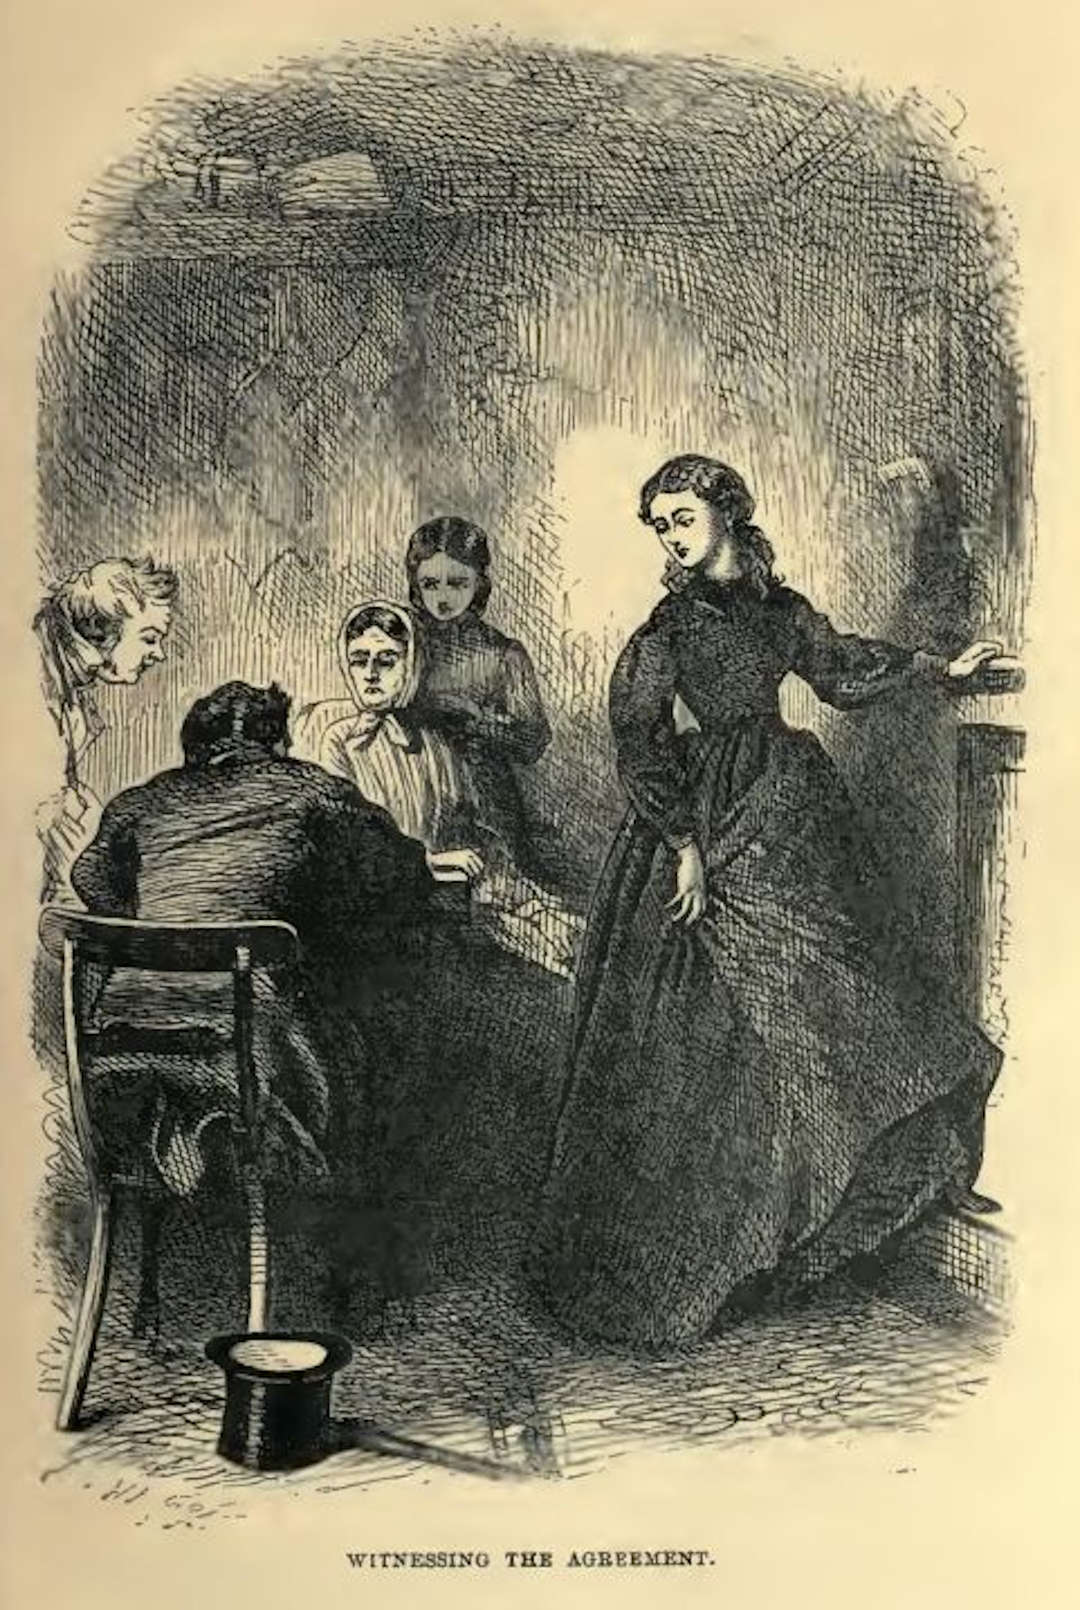
\includegraphics[scale=2.3]{01-04-01}

‘Much obliged to you, Miss Wilfer.’

‘Obliged?’

‘I have given you so much trouble.’

‘Signing my name? Yes, certainly. But I am your landlord’s daughter,
sir.’

As there was nothing more to do but pay eight sovereigns in earnest of
the bargain, pocket the agreement, appoint a time for the arrival of his
furniture and himself, and go, Mr Rokesmith did that as awkwardly as it
might be done, and was escorted by his landlord to the outer air. When
R. Wilfer returned, candlestick in hand, to the bosom of his family, he
found the bosom agitated.

‘Pa,’ said Bella, ‘we have got a Murderer for a tenant.’

‘Pa,’ said Lavinia, ‘we have got a Robber.’

‘To see him unable for his life to look anybody in the face!’ said
Bella. ‘There never was such an exhibition.’

‘My dears,’ said their father, ‘he is a diffident gentleman, and I
should say particularly so in the society of girls of your age.’

‘Nonsense, our age!’ cried Bella, impatiently. ‘What’s that got to do
with him?’

‘Besides, we are not of the same age:--which age?’ demanded Lavinia.

‘Never YOU mind, Lavvy,’ retorted Bella; ‘you wait till you are of an
age to ask such questions. Pa, mark my words! Between Mr Rokesmith and
me, there is a natural antipathy and a deep distrust; and something will
come of it!’

‘My dear, and girls,’ said the cherub-patriarch, ‘between Mr Rokesmith
and me, there is a matter of eight sovereigns, and something for supper
shall come of it, if you’ll agree upon the article.’

This was a neat and happy turn to give the subject, treats being rare in
the Wilfer household, where a monotonous appearance of Dutch-cheese at
ten o’clock in the evening had been rather frequently commented on by
the dimpled shoulders of Miss Bella. Indeed, the modest Dutchman himself
seemed conscious of his want of variety, and generally came before the
family in a state of apologetic perspiration. After some discussion on
the relative merits of veal-cutlet, sweetbread, and lobster, a decision
was pronounced in favour of veal-cutlet. Mrs Wilfer then solemnly
divested herself of her handkerchief and gloves, as a preliminary
sacrifice to preparing the frying-pan, and R. W. himself went out
to purchase the viand. He soon returned, bearing the same in a fresh
cabbage-leaf, where it coyly embraced a rasher of ham. Melodious sounds
were not long in rising from the frying-pan on the fire, or in seeming,
as the firelight danced in the mellow halls of a couple of full bottles
on the table, to play appropriate dance-music.

The cloth was laid by Lavvy. Bella, as the acknowledged ornament of the
family, employed both her hands in giving her hair an additional
wave while sitting in the easiest chair, and occasionally threw in a
direction touching the supper: as, ‘Very brown, ma;’ or, to her sister,
‘Put the saltcellar straight, miss, and don’t be a dowdy little puss.’

Meantime her father, chinking Mr Rokesmith’s gold as he sat expectant
between his knife and fork, remarked that six of those sovereigns came
just in time for their landlord, and stood them in a little pile on the
white tablecloth to look at.

‘I hate our landlord!’ said Bella.

But, observing a fall in her father’s face, she went and sat down by him
at the table, and began touching up his hair with the handle of a fork.
It was one of the girl’s spoilt ways to be always arranging the family’s
hair--perhaps because her own was so pretty, and occupied so much of her
attention.

‘You deserve to have a house of your own; don’t you, poor pa?’

‘I don’t deserve it better than another, my dear.’

‘At any rate I, for one, want it more than another,’ said Bella, holding
him by the chin, as she stuck his flaxen hair on end, ‘and I grudge
this money going to the Monster that swallows up so much, when we all
want--Everything. And if you say (as you want to say; I know you want
to say so, pa) “that’s neither reasonable nor honest, Bella,” then I
answer, “Maybe not, pa--very likely--but it’s one of the consequences
of being poor, and of thoroughly hating and detesting to be poor, and
that’s my case.” Now, you look lovely, pa; why don’t you always wear
your hair like that? And here’s the cutlet! If it isn’t very brown, ma,
I can’t eat it, and must have a bit put back to be done expressly.’

However, as it was brown, even to Bella’s taste, the young lady
graciously partook of it without reconsignment to the frying-pan, and
also, in due course, of the contents of the two bottles: whereof
one held Scotch ale and the other rum. The latter perfume, with
the fostering aid of boiling water and lemon-peel, diffused itself
throughout the room, and became so highly concentrated around the warm
fireside, that the wind passing over the house roof must have rushed off
charged with a delicious whiff of it, after buzzing like a great bee at
that particular chimneypot.

‘Pa,’ said Bella, sipping the fragrant mixture and warming her favourite
ankle; ‘when old Mr Harmon made such a fool of me (not to mention
himself, as he is dead), what do you suppose he did it for?’

‘Impossible to say, my dear. As I have told you time out of number since
his will was brought to light, I doubt if I ever exchanged a hundred
words with the old gentleman. If it was his whim to surprise us, his
whim succeeded. For he certainly did it.’

‘And I was stamping my foot and screaming, when he first took notice of
me; was I?’ said Bella, contemplating the ankle before mentioned.

‘You were stamping your little foot, my dear, and screaming with your
little voice, and laying into me with your little bonnet, which you
had snatched off for the purpose,’ returned her father, as if the
remembrance gave a relish to the rum; ‘you were doing this one Sunday
morning when I took you out, because I didn’t go the exact way you
wanted, when the old gentleman, sitting on a seat near, said, “That’s a
nice girl; that’s a VERY nice girl; a promising girl!” And so you were,
my dear.’

‘And then he asked my name, did he, pa?’

‘Then he asked your name, my dear, and mine; and on other Sunday
mornings, when we walked his way, we saw him again, and--and really
that’s all.’

As that was all the rum and water too, or, in other words, as R. W.
delicately signified that his glass was empty, by throwing back his head
and standing the glass upside down on his nose and upper lip, it might
have been charitable in Mrs Wilfer to suggest replenishment. But that
heroine briefly suggesting ‘Bedtime’ instead, the bottles were put away,
and the family retired; she cherubically escorted, like some severe
saint in a painting, or merely human matron allegorically treated.

‘And by this time to-morrow,’ said Lavinia when the two girls were alone
in their room, ‘we shall have Mr Rokesmith here, and shall be expecting
to have our throats cut.’

‘You needn’t stand between me and the candle for all that,’ retorted
Bella. ‘This is another of the consequences of being poor! The idea of a
girl with a really fine head of hair, having to do it by one flat candle
and a few inches of looking-glass!’

‘You caught George Sampson with it, Bella, bad as your means of dressing
it are.’

‘You low little thing. Caught George Sampson with it! Don’t talk about
catching people, miss, till your own time for catching--as you call
it--comes.’

‘Perhaps it has come,’ muttered Lavvy, with a toss of her head.

‘What did you say?’ asked Bella, very sharply. ‘What did you say, miss?’

Lavvy declining equally to repeat or to explain, Bella gradually lapsed
over her hair-dressing into a soliloquy on the miseries of being poor,
as exemplified in having nothing to put on, nothing to go out in,
nothing to dress by, only a nasty box to dress at instead of a
commodious dressing-table, and being obliged to take in suspicious
lodgers. On the last grievance as her climax, she laid great stress--and
might have laid greater, had she known that if Mr Julius Handford had a
twin brother upon earth, Mr John Rokesmith was the man.






(TO BE CONTINUED)

% %%%%%%%%%%%%
\end{document}%
% End of document.
% %%%%%%%%%%%%%%%%


